% GENI Lab_2.tex - GENI Lab 1 for Cloud Computing class (Spring 2015)
% Chanmann Lim - March 2015

\documentclass[a4paper]{article}

\usepackage[margin=1 in]{geometry}
\usepackage{listings}
\usepackage{graphicx}
\usepackage{float}

\begin{document}
\title{CS 7001-03: Report for GENI Lab 2 - Instrumentation and Measurement of a GENI Slice}
\author{Chanmann Lim\\ 
	\texttt{cl9p8@mail.mail.missouri.edu}}
\date{March 10, 2015}
\maketitle

% ---------------------------------------- 1 ----------------------------------------
\paragraph{1. } Screenshots of OnTimeMeasure instance's Graphite page:
\begin{figure}[H]
  \centering
    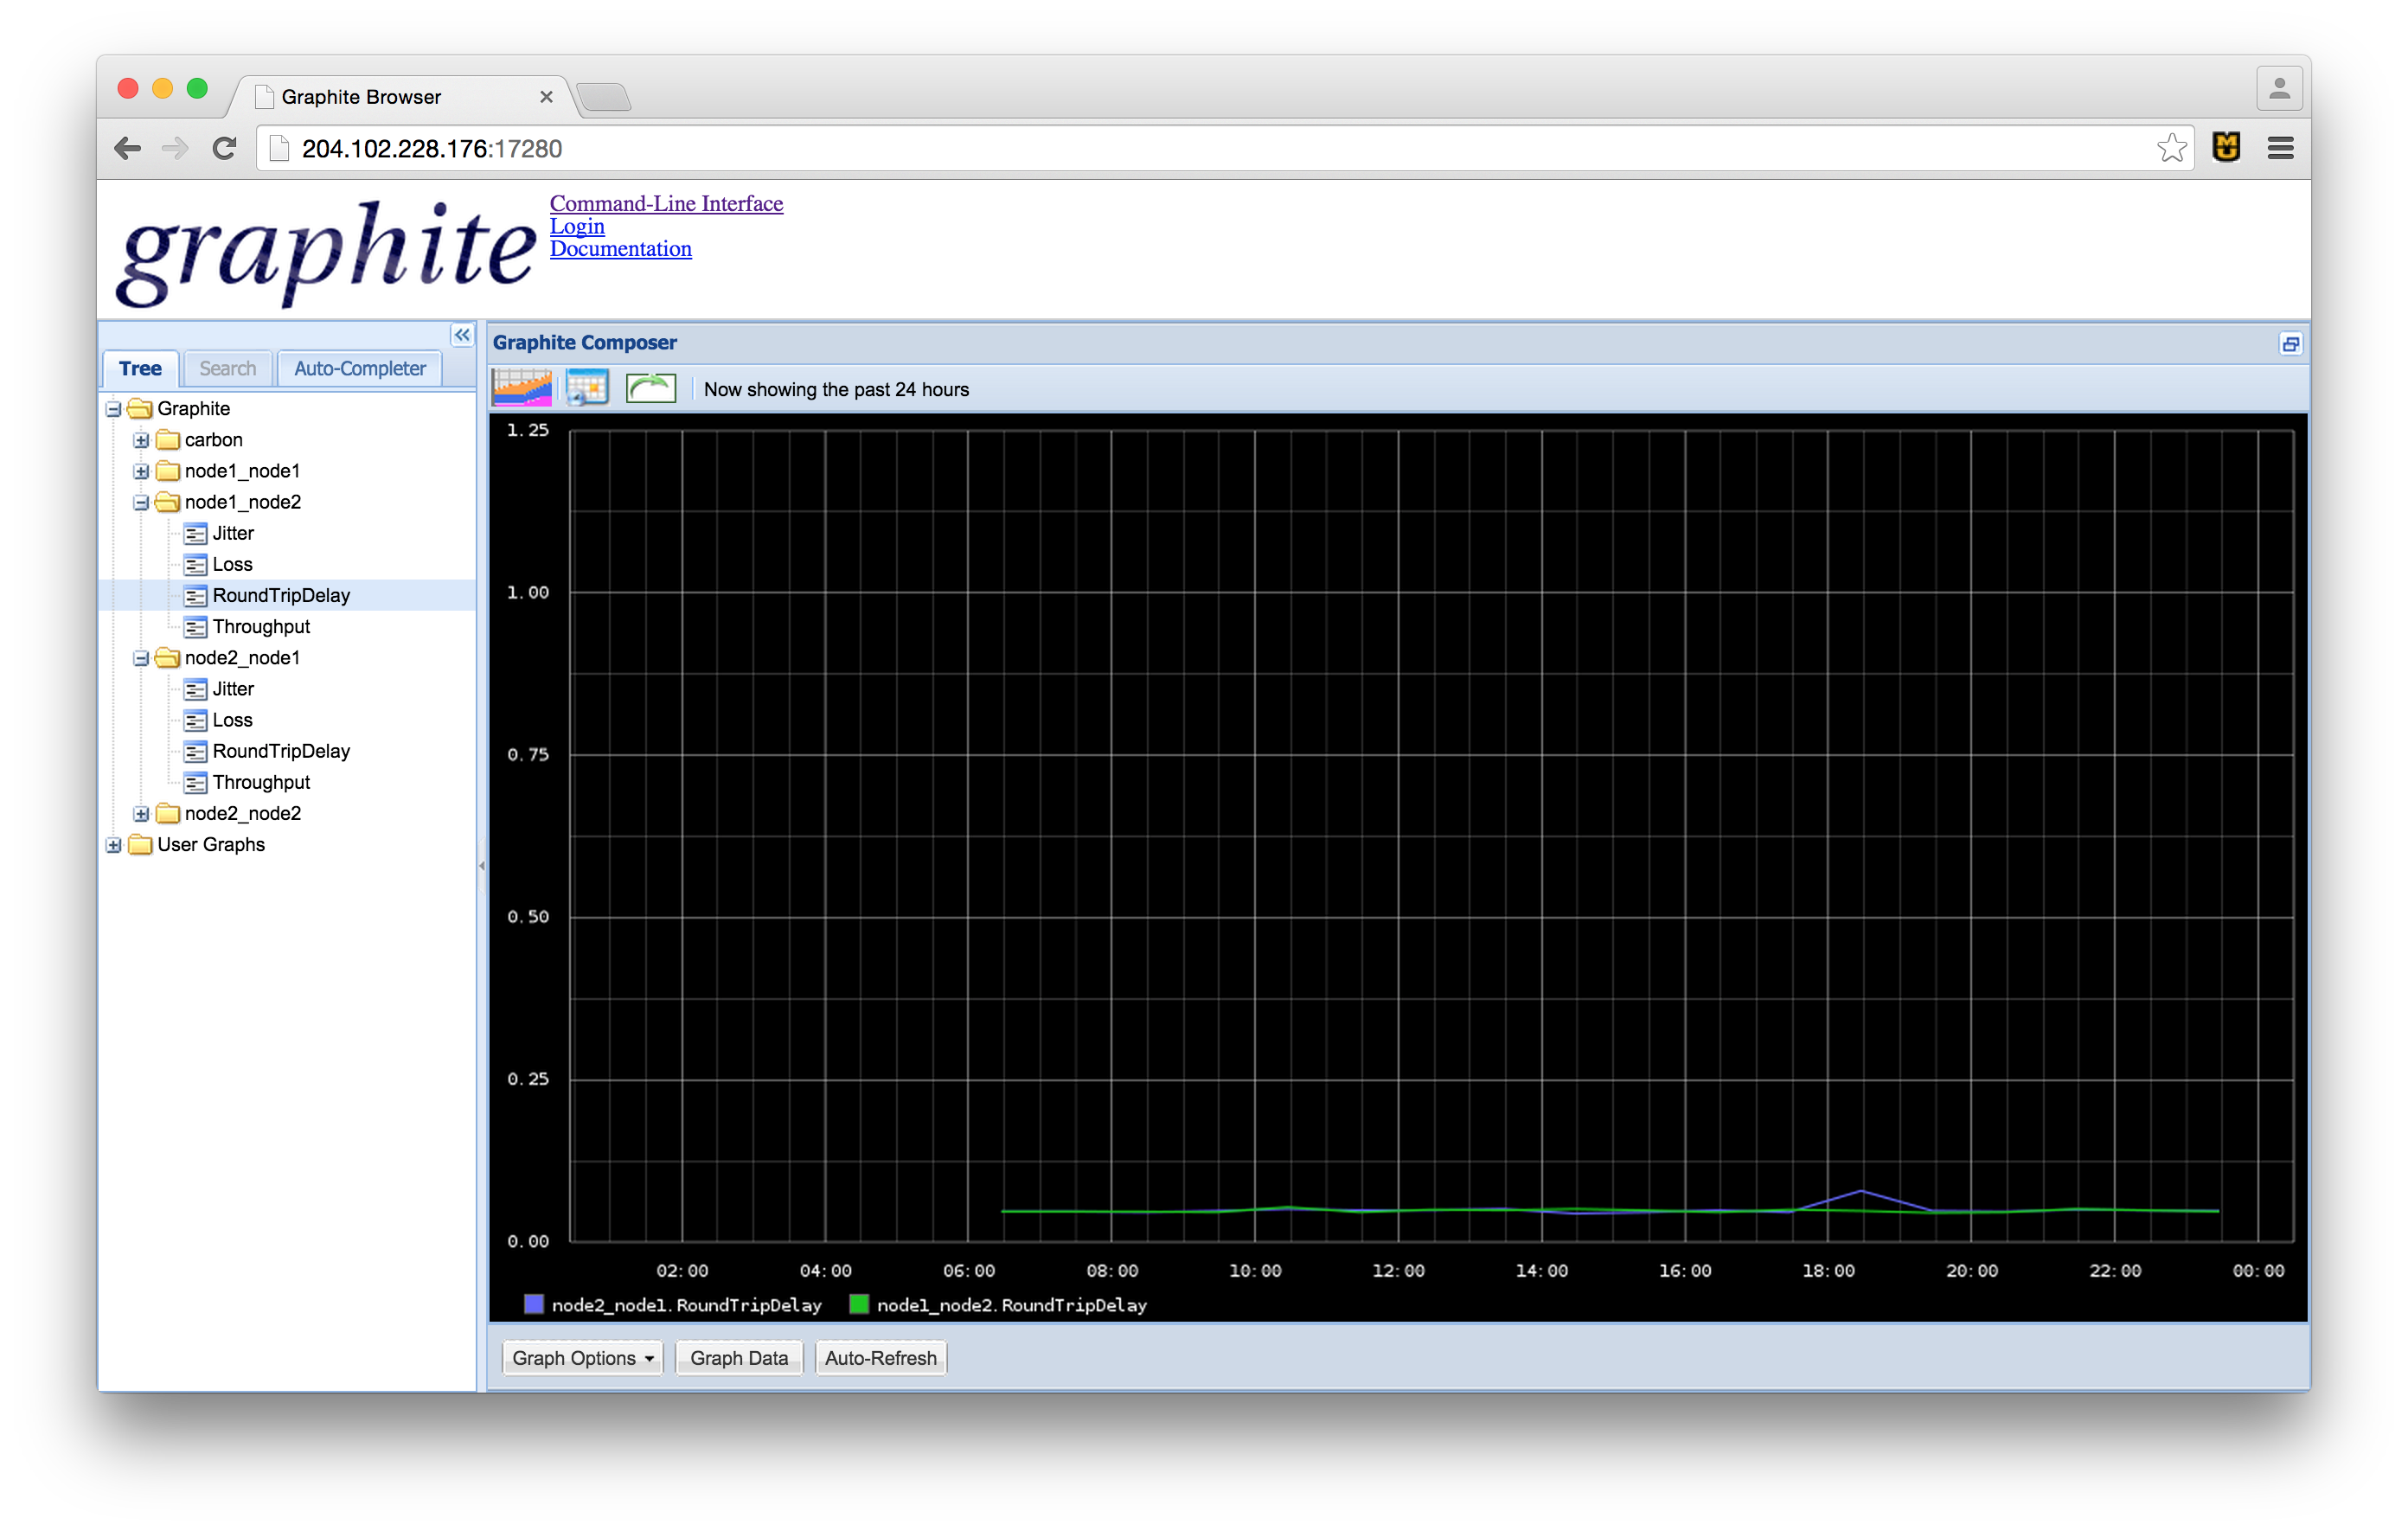
\includegraphics[scale=.32]{round_trip_delay.png}
  \caption{RoundTripDelay}
\end{figure}
\begin{figure}[H]
  \centering
    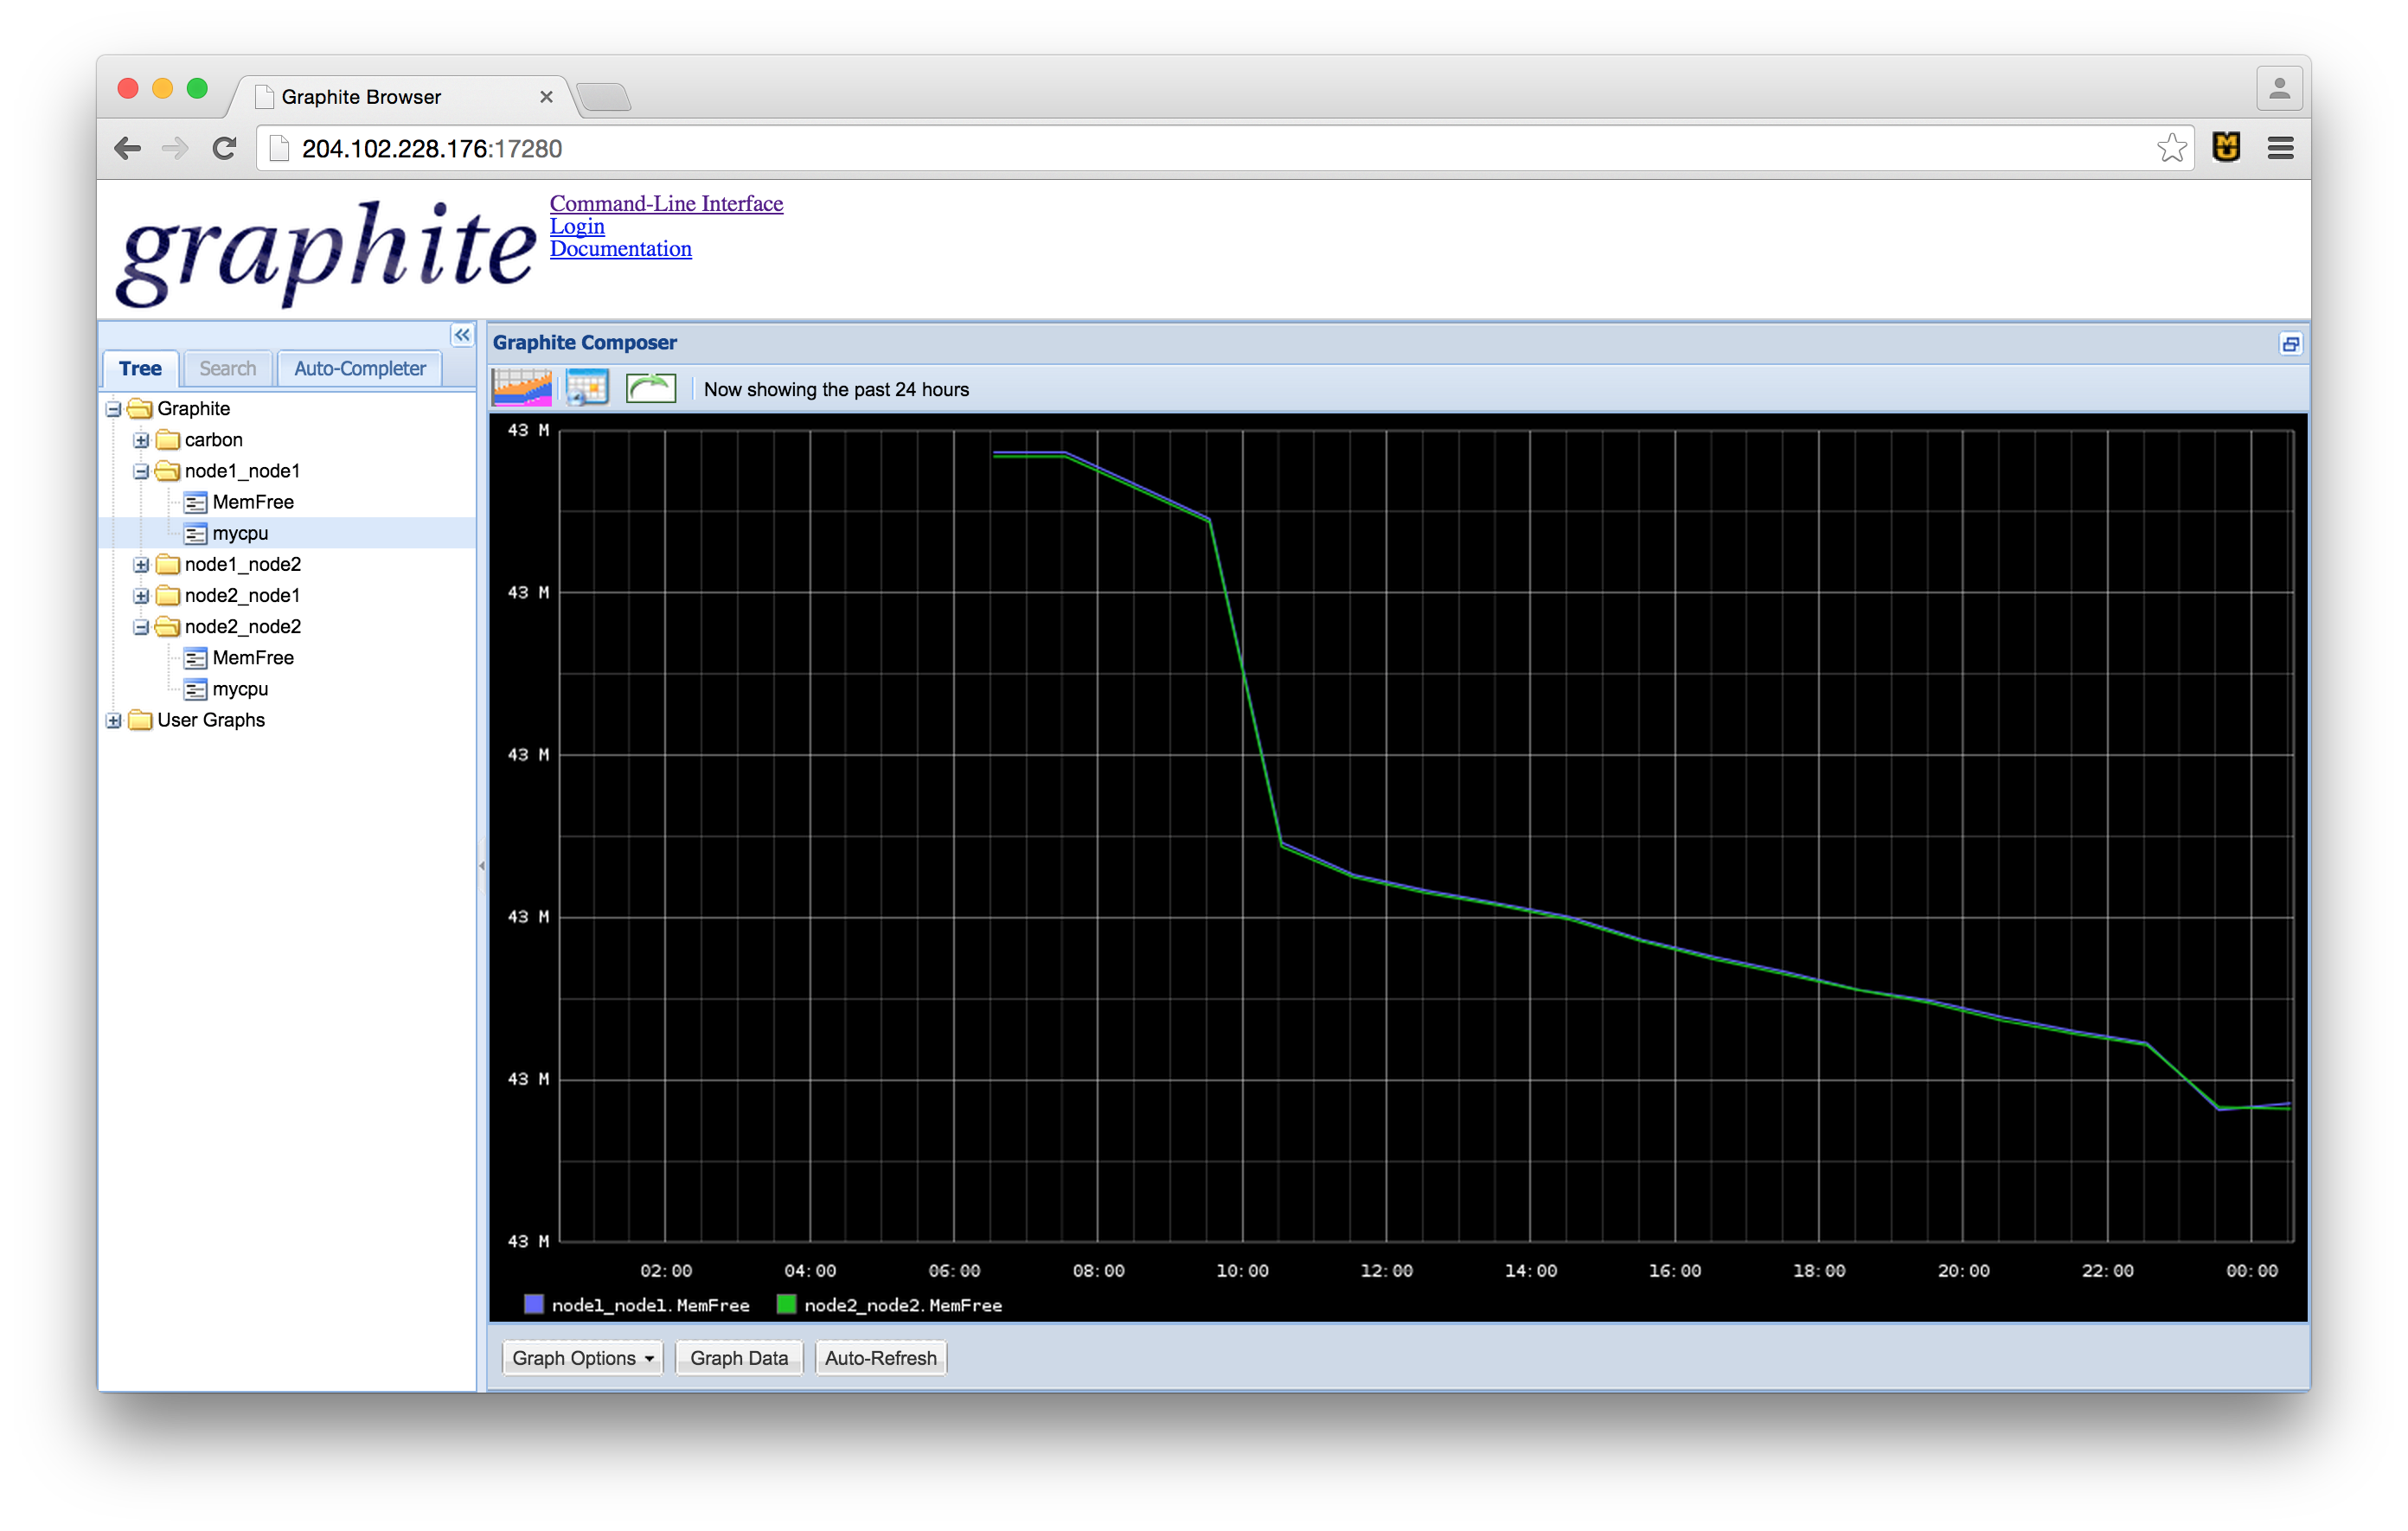
\includegraphics[scale=.32]{memfree.png}
  \caption{MemFree}
\end{figure}
\begin{figure}[H]
  \centering
    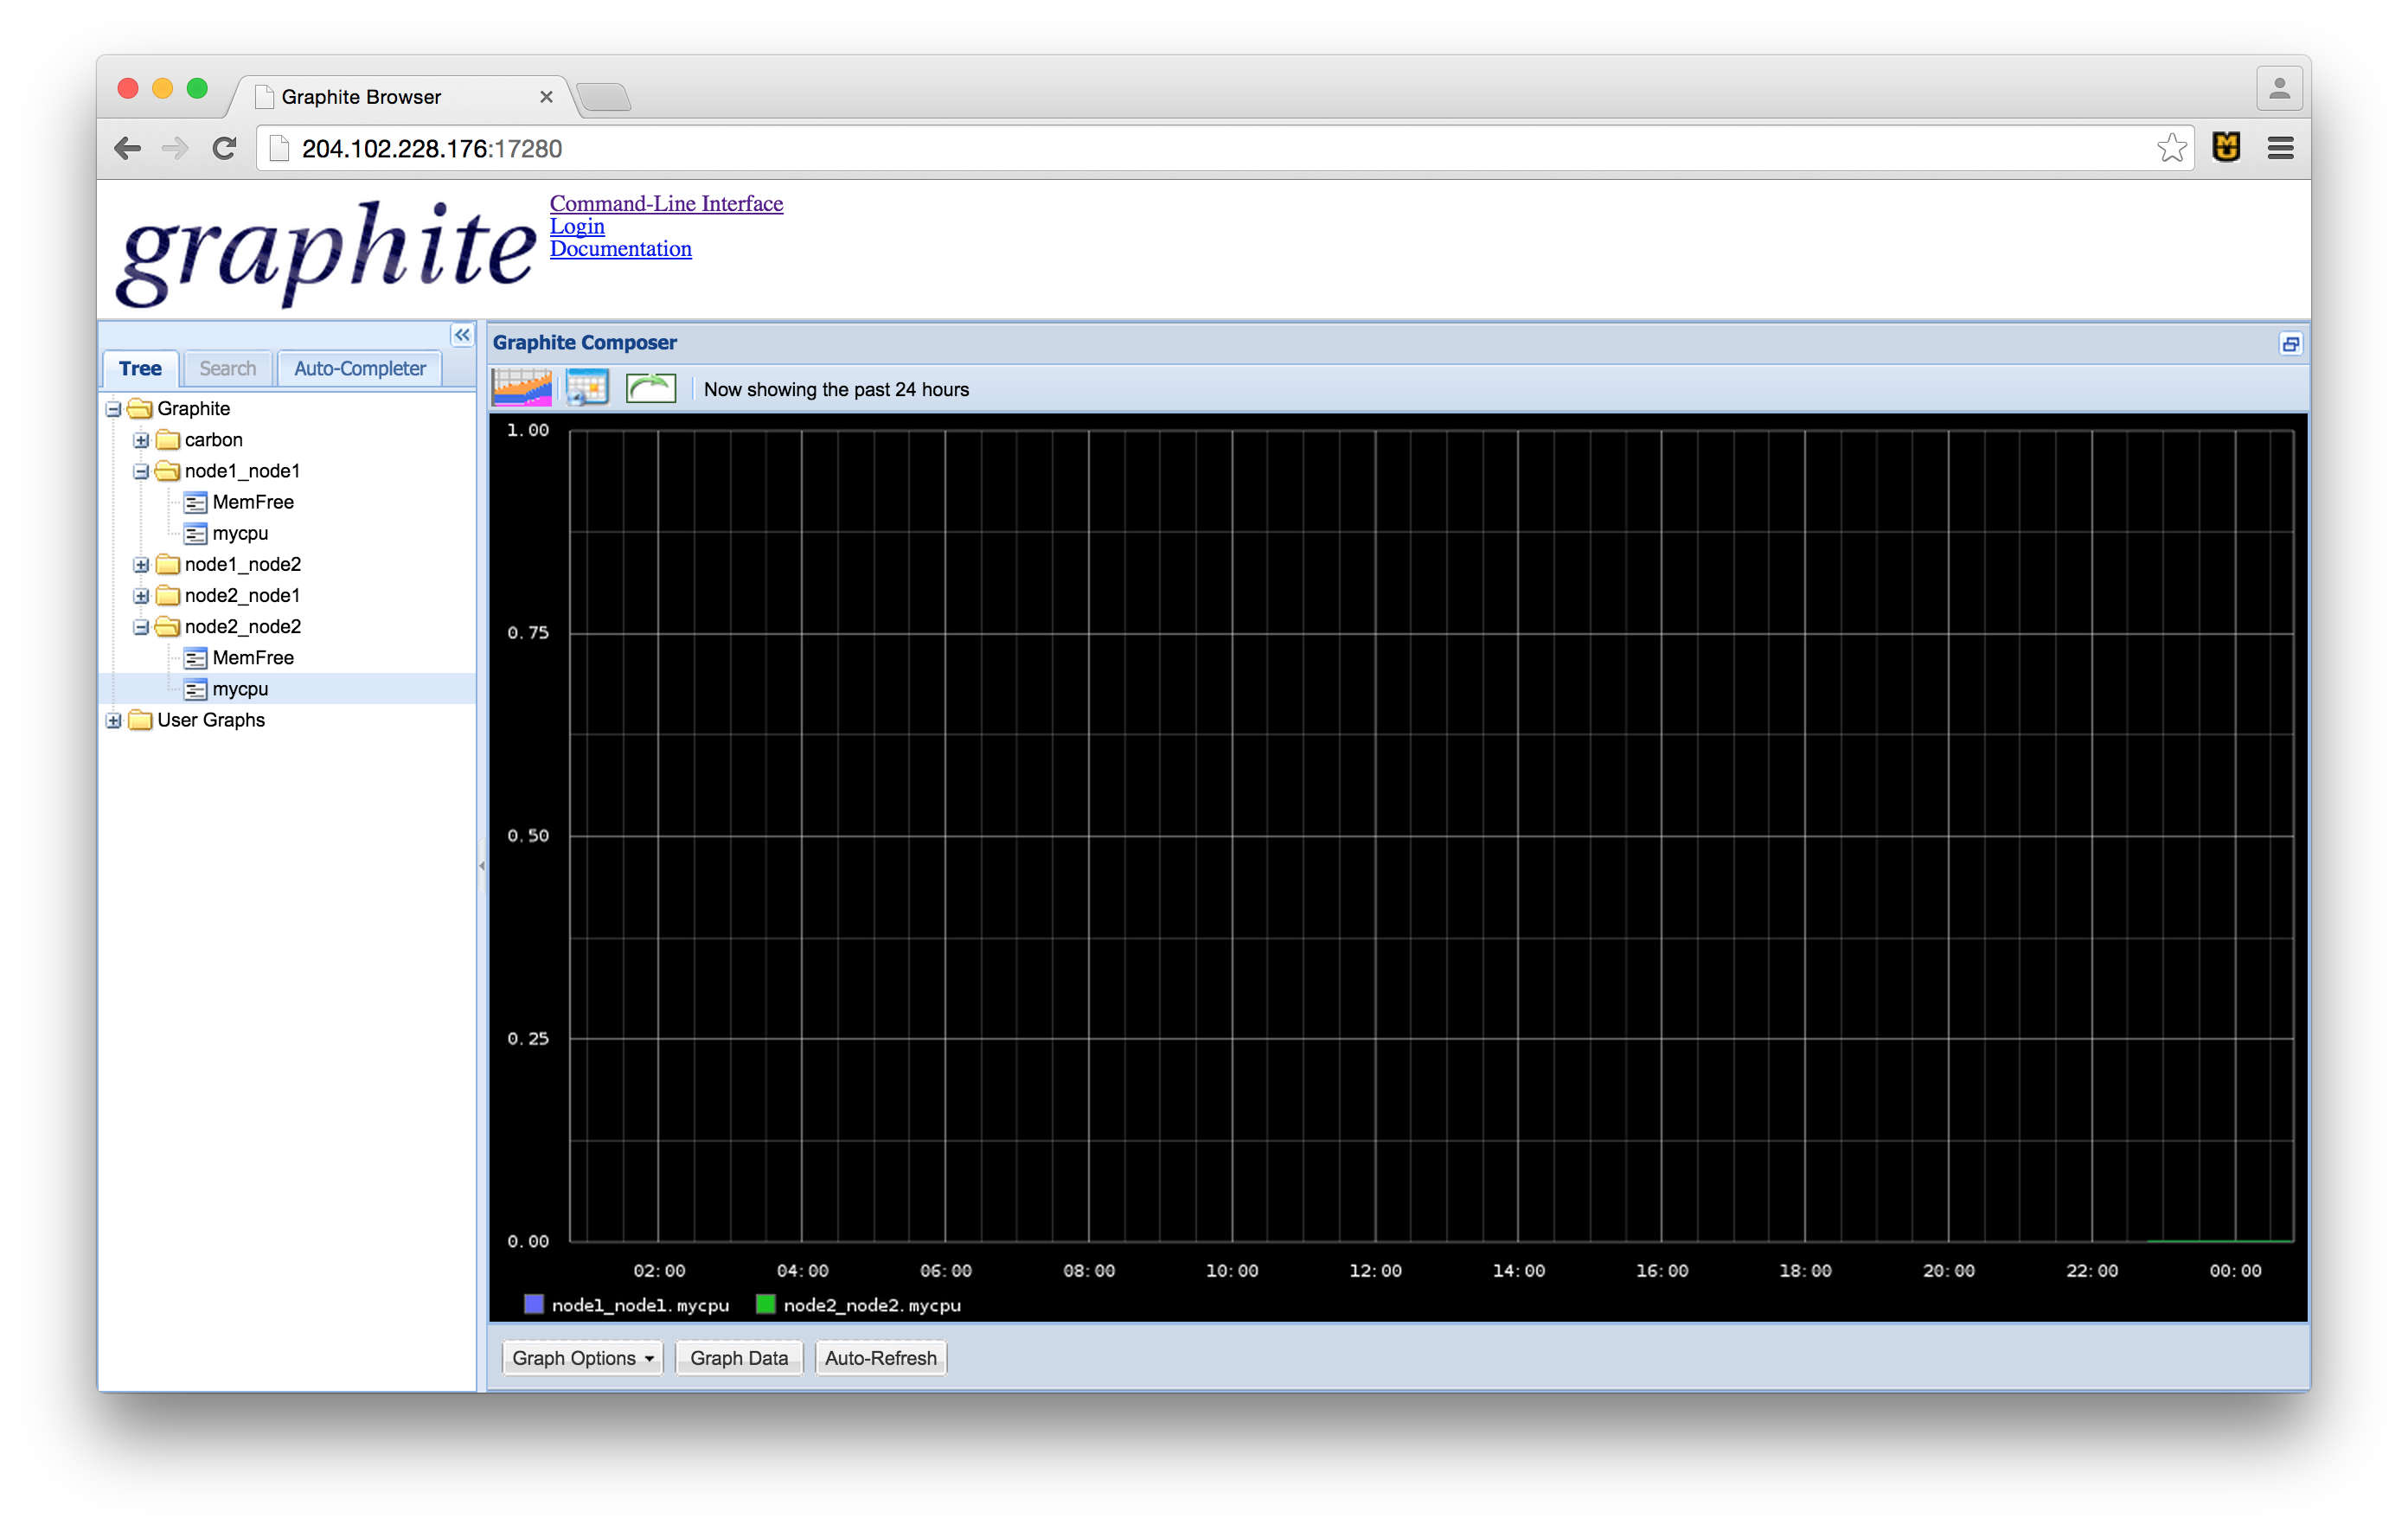
\includegraphics[scale=.32]{mycpu.png}
  \caption{MyCPU on node1 and node2}
\end{figure}

% ---------------------------------------- 2 ----------------------------------------
\paragraph{2. } Instrumentation and Measurement Tools such as \textbf{OnTimeMeasure} provides the on-going and on-demand measurement services used in network weather forecasting, path monitoring, performance anomaly detection and fault-location diagnosis in GENI experiments and GENI operations. \\
And \textbf{GEMINI} Tool set provides measurement services for both GENI experimenters and GENI infrastructure operators to collect, manage measurements metric and register measurement metadata and services with Unified Network Information Service (UNIS).

% ---------------------------------------- 3 ----------------------------------------
\paragraph{3. } \textbf{OnTimeControl} is the command-line interface client for \textbf{OnTimeMeasure}. First we need to have Root and Node beacons already have OnTimeMeasure installed and running on a GENI slice then OnTimeControl on the client machine is configured with yaml configuration file containing IP addresses of the root and node beacons, database password and portal connection and finally users use python interpreter to execute OnTimeControl python scripts to communicate with OnTimeMeasure.

% ---------------------------------------- 4 ----------------------------------------
\paragraph{4. } The workflow to add custom metric to OnTimeMeasure framework instance:
\begin{enumerate}
	\item Configure IP address and database password
	\begin{itemize}
		\item SSH login to the root beacon
		\item configure OnTimeControl
		\begin{itemize}
			\item navigate to \texttt{/opt/OnTimeMeasure/OnTimeControl}
			\item copy \texttt{config\_example.yaml} then paste as \texttt{config.yam}
			\item edit \texttt{config.yam} and change IP addresses of the root and nodes beacons, db\_pwd and portal configuration
		\end{itemize}
	\end{itemize}
	\item Install the custom metric on to the OnTimeMeasure Framework
	\begin{itemize}
		\item download the metric tool (e.g. \texttt{http://ontime.rnet.missouri.edu/INSTALL/metric/CPU.tgz}) and extract it
		\item execute \texttt{add\_metric.py} to add metric with the extracted specification file and parser file
		\item update measurement configuration file (\texttt{measurement.yaml}) to include the new metric
	\end{itemize}
	\item Restart the measurement service
\end{enumerate}
\end{document}